\documentclass[sn-mathphys]{sn-jnl}

\jyear{2022}%

\usepackage{lineno}
\modulolinenumbers[5]

\usepackage{lscape,pdflscape}

\usepackage{amsmath}
\usepackage{makeidx}  % allows for indexgeneration
\usepackage{graphicx}
\usepackage{url}
\usepackage{paralist}
%\usepackage[ruled,vlined,noresetcount]{algorithm2e}
\usepackage{bbding}

\usepackage{soul,color}
\sethlcolor{green}
\usepackage{xspace}

\usepackage{extarrows}
\usepackage{arydshln}

%\newtheorem{thm}{\textsc{Theorem}}
%\newtheorem{defs}{\textbf{Definition}}

\newtheorem{ex}{\textbf{Example}}


%\newcommand{\SO}{$^s\mathcal{O}$\xspace}
%\newcommand{\SDO}{$^s\mathcal{O}_d$\xspace}
%\newcommand{\SFO}{$^s\mathcal{O}_f$\xspace}
%\newcommand{\TO}{$^t\mathcal{O}$\xspace}
%\newcommand{\TDO}{$^t\mathcal{O}_d$\xspace}
%\newcommand{\TFO}{$^t\mathcal{O}_f$\xspace}

\newcommand{\crowd}{{\sf crowd}\xspace}
\newcommand{\crowdone}{{\sf crowd 1.0}\xspace}
\newcommand{\crowdtwo}{{\sf crowd 2.0}\xspace}

\newcommand{\bfkframe}{{\sf FaCIL}\xspace}

%\renewcommand{\baselinestretch}{.99}
%\input{macros}

\raggedbottom

\begin{document}

\title[A Framework for Interoperability Between Models with Hybrid Tools]{A Framework for Interoperability Between Models with Hybrid Tools: Use Case with \crowdtwo\footnote{Submitted to the Journal of Intelligent Information Systems}}


\author[1,2]{\fnm{Germán} \sur{Braun}}\email{german.braun@fi.uncoma.edu.ar}

\author[3,4]{\fnm{Pablo Rubén} \sur{Fillottrani}}\email{prf@cs.uns.edu.ar}
%\equalcont{These authors contributed equally to this work.}

\author[5]{\fnm{C. Maria} \sur{Keet}}\email{mkeet@cs.uct.ac.za}
%\equalcont{These authors contributed equally to this work.}

\affil[1]{Universidad Nacional del Comahue, Argentina}

\affil[2]{Consejo Nacional de Investigaciones Científicas y Técnicas, Argentina}

\affil[3]{Universidad Nacional del Sur, Argentina}

\affil[4]{Comisión de Investigaciones Científicas de la provincia de Buenos Aires, Argentina}

\affil[5]{Department of Computer Science, University of Cape Town, South Africa}


\maketitle


\section{Covid19 Use case with \crowdtwo}
\label{sec:usecase}

\begin{figure}%[b]
	\centering
		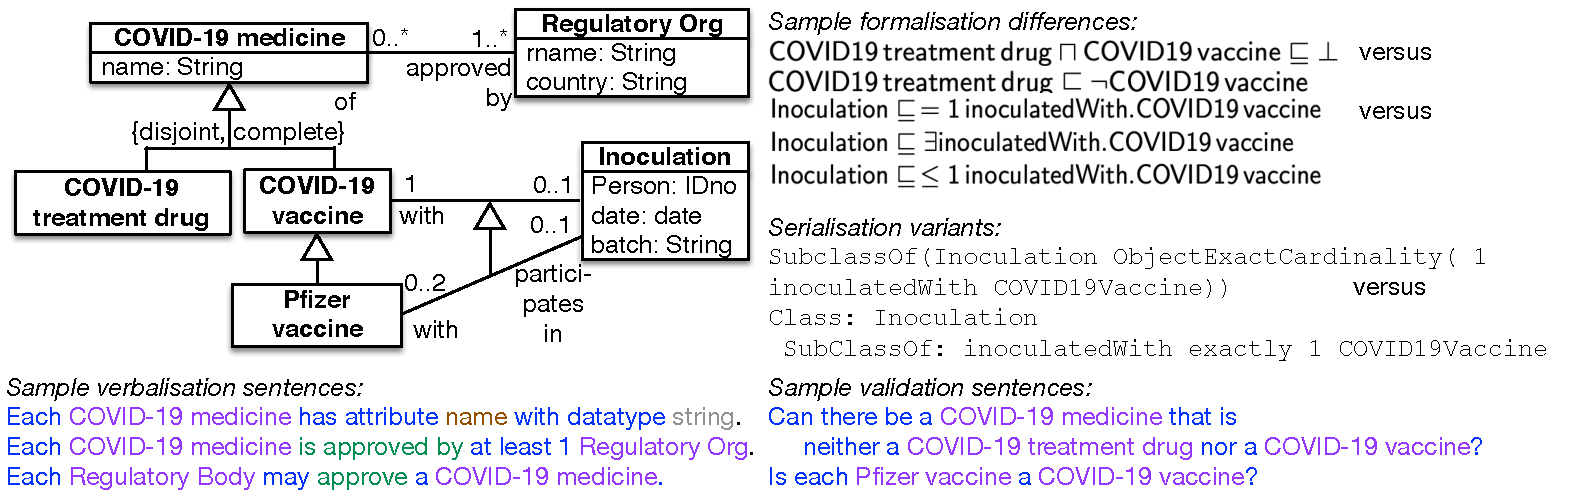
\includegraphics[width=\textwidth]{COVIDdrugsEx2.pdf}
	\caption{A selection of a possible conceptual model about COVID-19 medicines (suboptimal for illustrative purpose) and examples of formalisation and serialisation variants.}
	\label{fig:COVIDex}
\end{figure}

This document details motivational scenario about the modelling of the COVID-19 medicines in Fig \ref{fig:COVIDex} with the tool \crowdtwo. To do this, we will follow the use case depicted in Fig.~\ref{fig:usecase}, which illustrates how users can work collaboratively by exploring a conceptual model from different perspectives that suit their respective competencies and core tasks. %Some screenshots are included here, while other ones are provided as supplementary material accompanying this submission.

\begin{figure}[h]
  \centering
   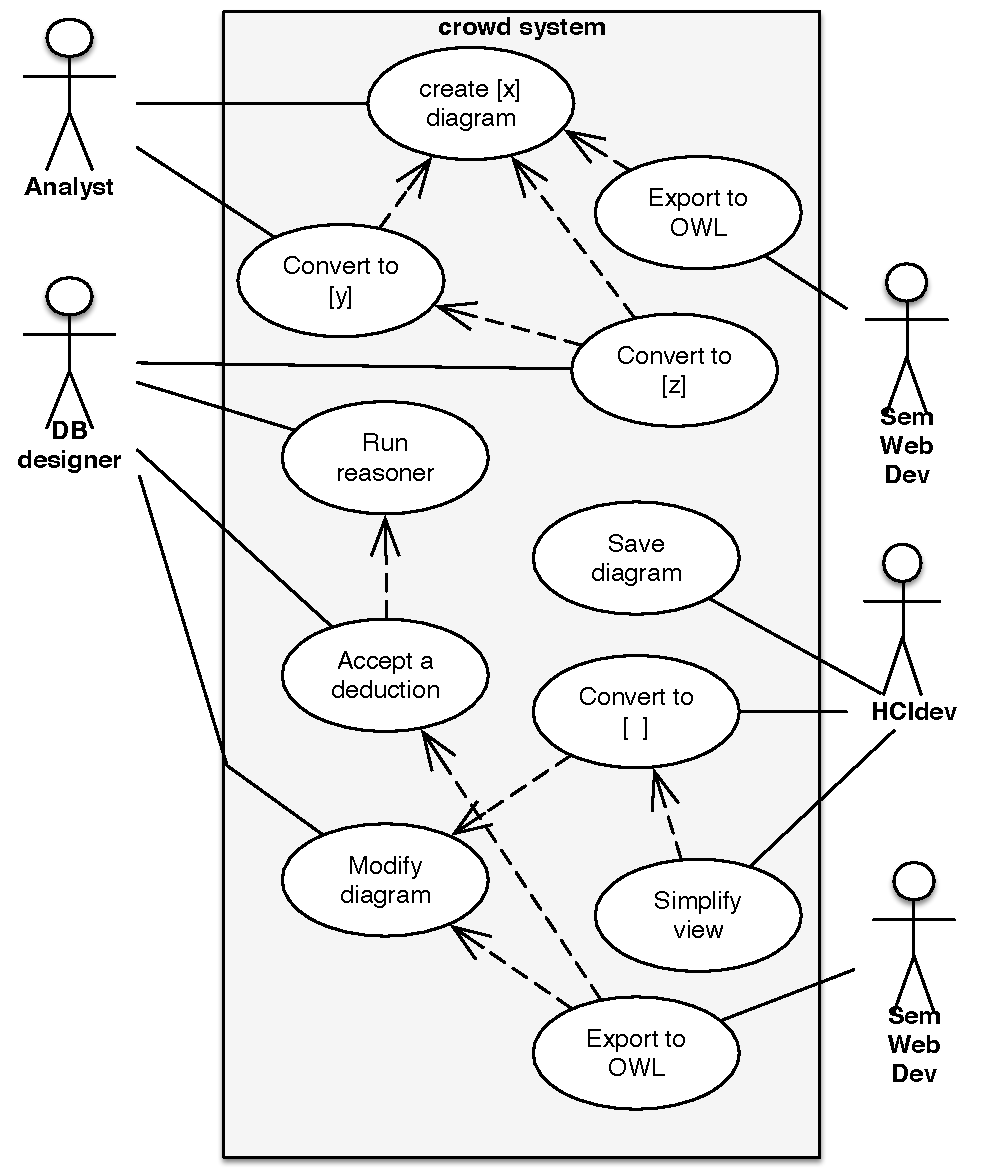
\includegraphics[width=0.7\textwidth]{COVIDdrugsProcessFlowEx2.pdf} 
    \caption{Sample use case diagram related to the use case described in Section~\ref{sec:usecase} The [x], [y] and [z] are distinct and either UML, EER, and ORM; the ``[ ]'' is UML in the use case, but each type of diagram can be simplified and so left blank here.}
    \label{fig:usecase}
\end{figure}

\begin{figure}[h]
  \centering
   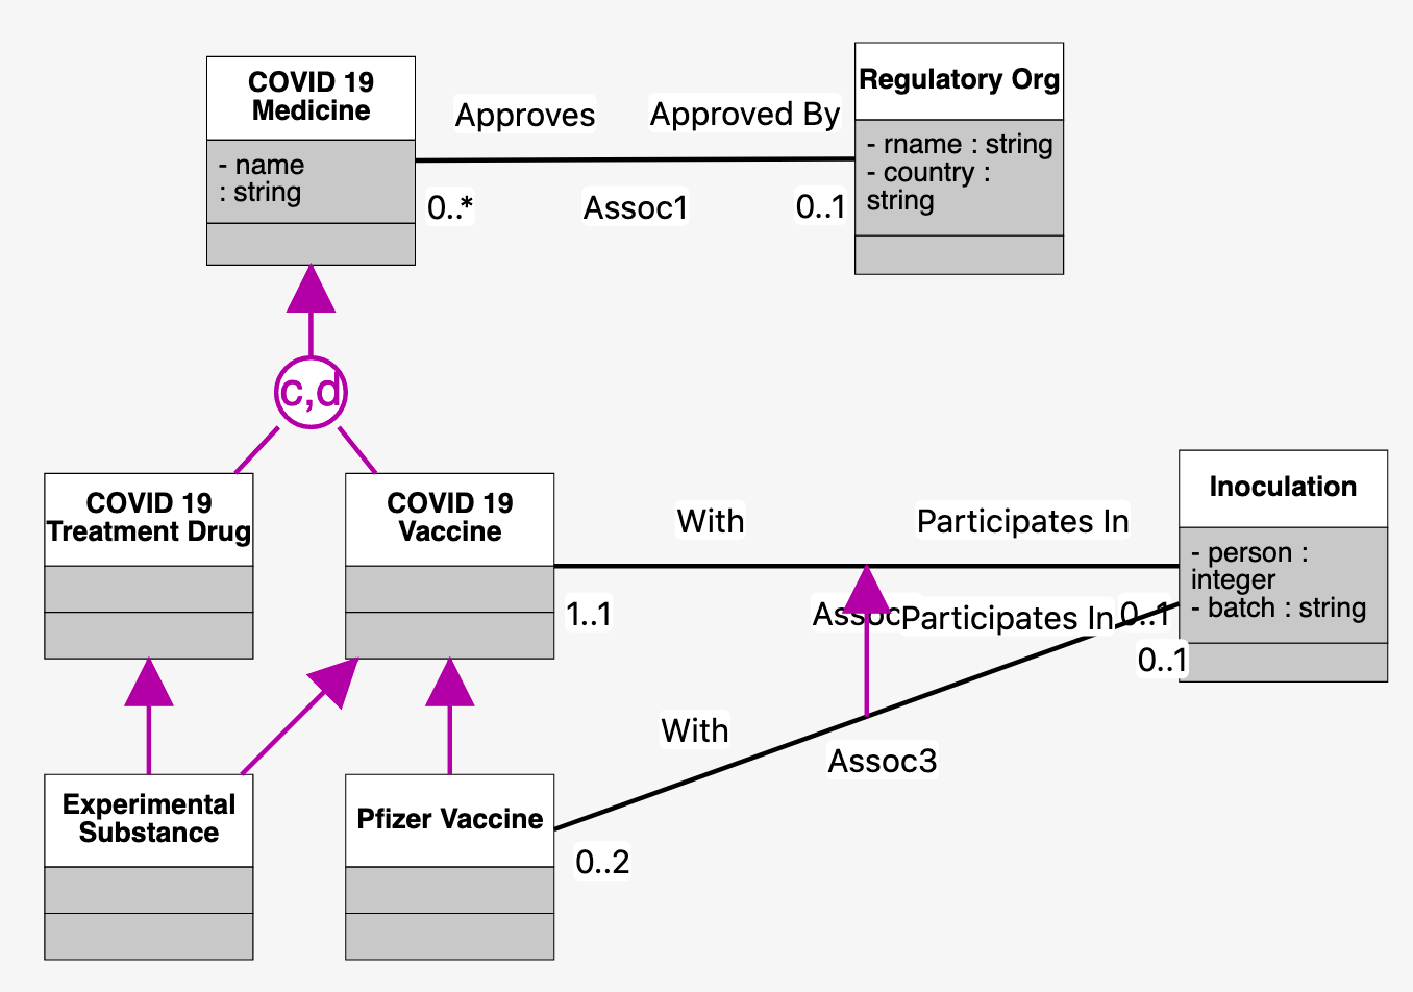
\includegraphics[width=0.9\textwidth]{covidUML1.pdf} 
    \caption{The same UML diagram as in Fig.~\ref{fig:COVIDex}, but then rendered in \crowdtwo's interface.}
    \label{fig:UML}
\end{figure}

First, let us put the UML diagram into \crowdtwo (see Fig.~\ref{fig:UML}). To push the tool's capabilities a little more so as to obtain more interesting results, we add an additional class in the spirit of the CIDO ontology\footnote{\url{https://www.ebi.ac.uk/ols/ontologies/cido}}, called {\sf Experimental substance}, which is also shown in Fig.~\ref{fig:UML}. Its back-end runtime conceptual model as KF instantiation and the implementation of the rules were then called to generate automatically their corresponding EER and ORM2 versions, which are depicted in Fig.~\ref{fig:ERandORM}. As can be seen in the figures, there are labels like {\sf Assoc3} (abbreviated from the default generated {\sf Association-x}, where x is an increment count in the interface) and  {\sf Qf Wzz9} in Fig.~\ref{fig:ERandORM}: EER requires names for relationships, but UML does not, and this discrepancy is fixed with default naming. This is similar for ORM2, where  a UML attribute is converted into a ORM2 value type that uses an extra mandatory 1:1 fact type (relationship) for it, which have been added. They all can be modified by the modeller.


\begin{figure}[h]
  \centering
   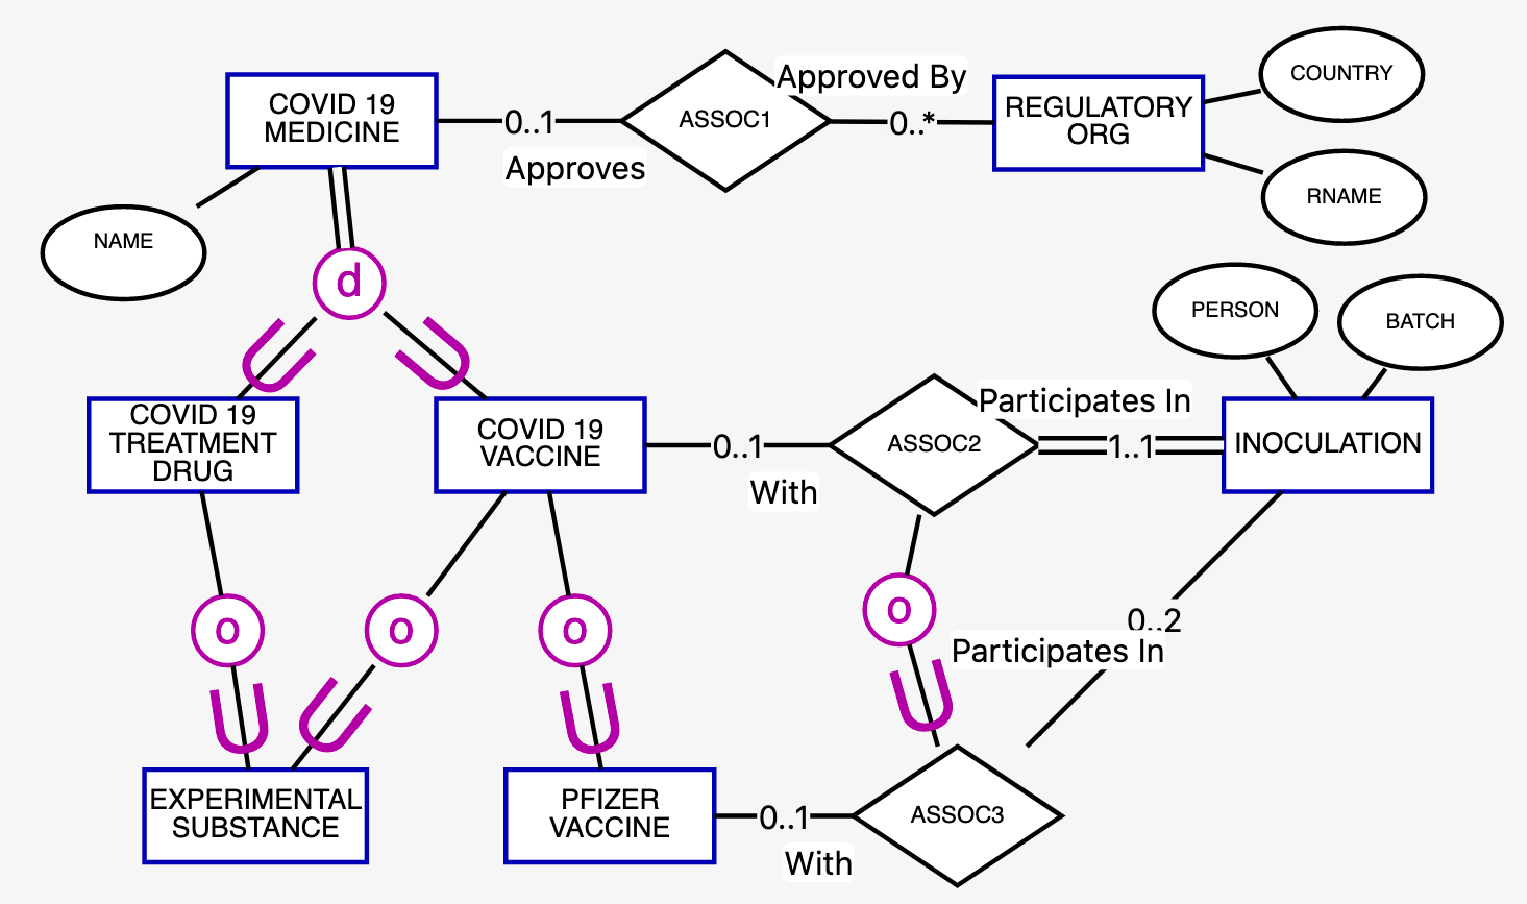
\includegraphics[width=0.95\textwidth]{covidER1.pdf} 
   
         \vspace{1mm}
         
         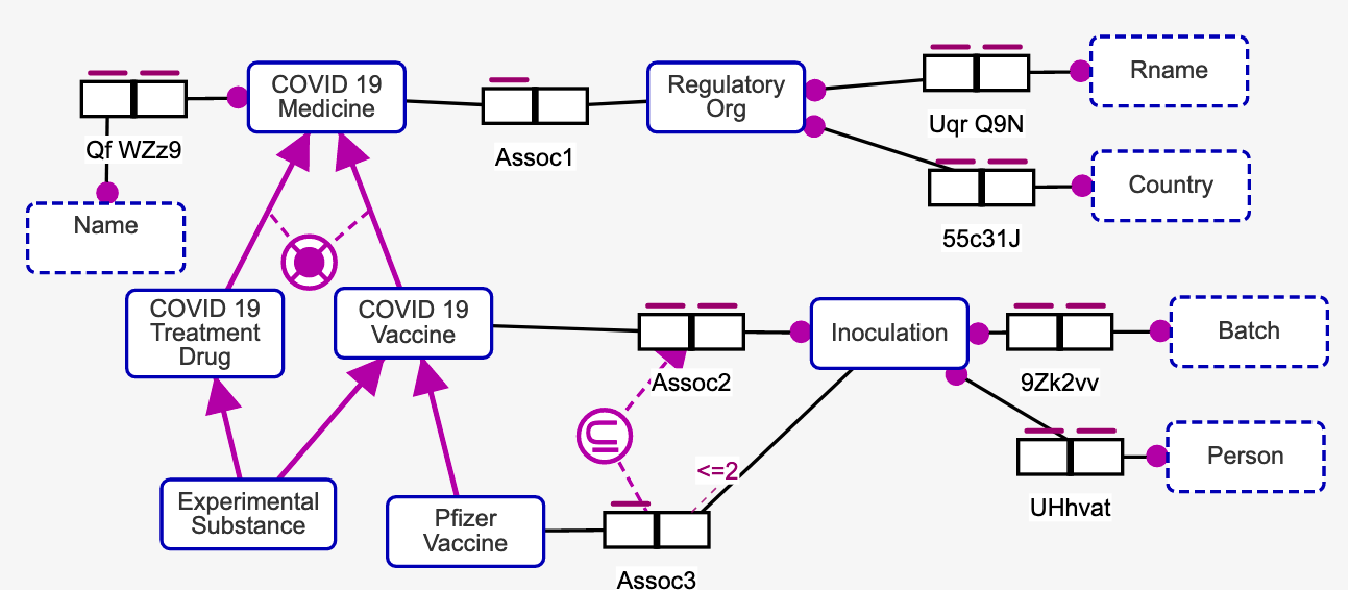
\includegraphics[width=0.95\textwidth]{covidORM1.pdf} 
         
    \caption{Automatically generated EER and ORM diagram versions of the original UML class diagram model of Fig.~\ref{fig:UML}.}
    \label{fig:ERandORM}
\end{figure}

Let's assume the modeller is a database analyst, and so we present them the EER diagram. They decide to run the reasoner over the EER diagram to double-check its quality. The deductions are displayed visually as shown in Fig.~\ref{fig:ER1reasoner} and, upon clicking it, a brief note appears in the right-hand pane of the tool, as shown in the two fragments in Fig.~\ref{fig:ER1reasonerexplain}:  {\sf Experimental substance} is unsatisifiable because its parent classes are disjoint and the cardinality on the {\sf Pfizer vaccine} changed from {\sf 0..2} to {\sf 0..1} because of the cardinality on {\sf with} in {\sf Assoc2} and the subsetting constraint on the relationships. The modeller can accept or reject the deductions.


\begin{figure}[h]
  \centering
      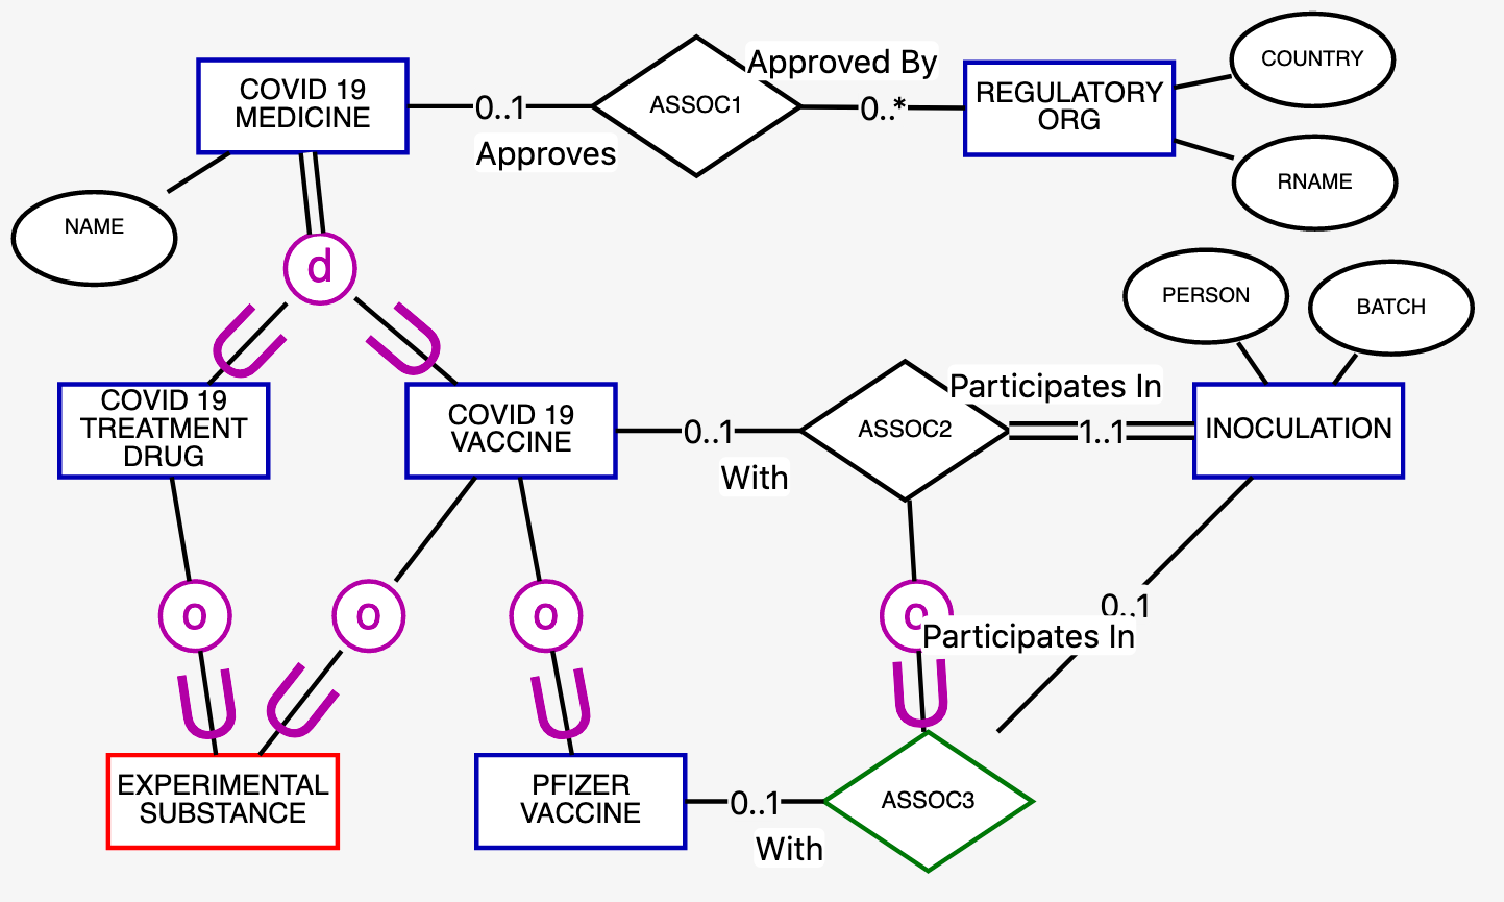
\includegraphics[width=0.95\textwidth]{covidER1reasoneroutput.pdf} 
    \caption{Deductions over the model, obtained with the automated reasoner: {\sf Experimental substance} is unsatisfiable and the cardinality on the {\sf Pfizer vaccine} changed from {\sf 0..2} to {0..1}.}
    \label{fig:ER1reasoner}
\end{figure}

\begin{figure}[h]
  \centering
      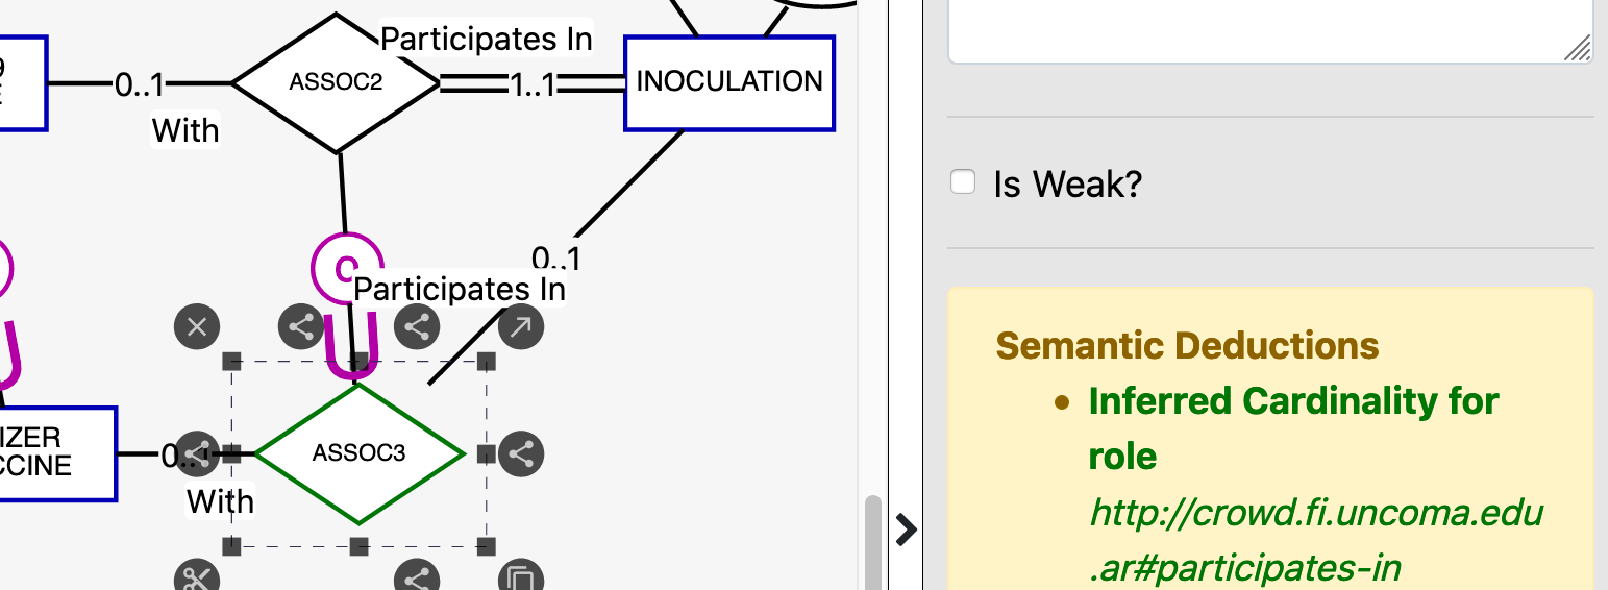
\includegraphics[width=0.95\textwidth]{covidER1card.pdf} 
      
      \vspace{1mm}
      
            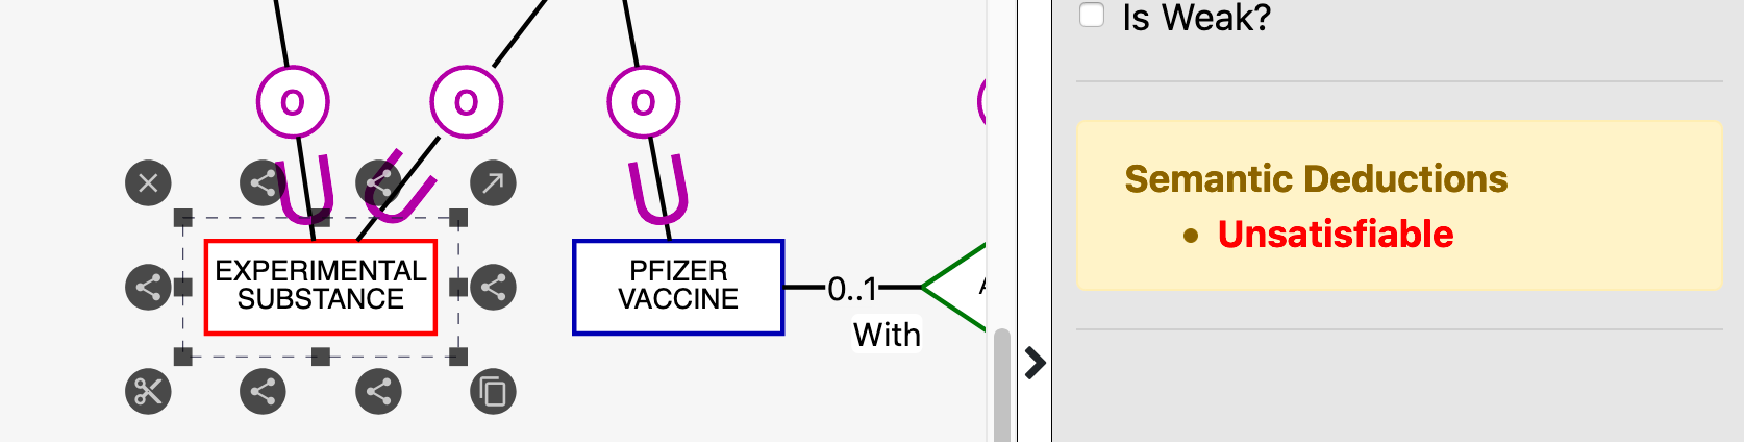
\includegraphics[width=0.95\textwidth]{covidER1unsat.pdf} 
            
    \caption{Clicking on the coloured elements of the model (included in Fig.~\ref{fig:ER1reasoner}) provides some detail in the right-hand pane for both deduction}
    \label{fig:ER1reasonerexplain}
\end{figure}

The database analyst is actually more of an expert in ORM and for now rejects the deductions, automatically transforms the EER diagram into an ORM diagram, and runs the reasoner again. The same deductions are displayed visually. The analyst is now more confident about the deduction on the cardinality constraint on  {\sf Pfizer vaccine} and accepts that deduction. They also remember to add that the regulatory organisation {\sf coordinates} the {\sf Inoculation}, and modify the model accordingly. Since their colleague actually does prefer EER, they convert it back to EER, which is shown in Fig.~\ref{fig:ORM2toER} with the relevant section in the GUI of \crowdtwo (for purpose of readability and layout, these and the following figures are included at the end of the paper in the appendix). There was still that {\sf Experimental substance} to deal with, and the EER diagram is modified by deleting that unsatisfiable class. A third colleague, in HCIdev group, prefers UML class diagram notation of front-end app development and so it is transformed back into one (Fig.~\ref{fig:ER2toUML}), which, cf. the model we started with, has been updated with the changes that were made to the model when it was an ORM and an EER diagram before. 

This UML diagram still can be modified just like it was done with the other two models in the other notations, which then also correspondingly updates the runtime conceptual model and its serialisation in JSON. A section of the JSON serialisation is depicted in Fig.~\ref{fig:UMLmod}. Then, to generate a more compact diagram for an easier overview, the HCIdev modeller can choose to `declutter' it by toggling the attributes/methods and the role and relationship names, so as to obtain a simplified visual notation whilst maintaining the details in the background (Fig.~\ref{fig:UMLabstract}). %\nb{we need to add the CNL option} 
Also, upon the client's request for validating the model, the HCIdev employee generates a text-based version with an English CNL (see Fig.~\ref{fig:toCNL}). %\nb{G: fig added}

Finally, to not lose all the work done, any of the modellers involved can save and, optionally also, export it from \crowdtwo. The tool saves the model in JSON, which is specific to each CDML (see Fig.~\ref{fig:jsonER2andUML2}), so as to serialise and persistently store the instantiation of the KF metamodel (see Fig.~\ref{fig:toKF}). It can export it to OWL  (see Fig.~\ref{fig:toOWL}) so that it also can be used in an ontology-driven information system that relies on Semantic Web technologies.

\begin{figure}[h]
  \centering
      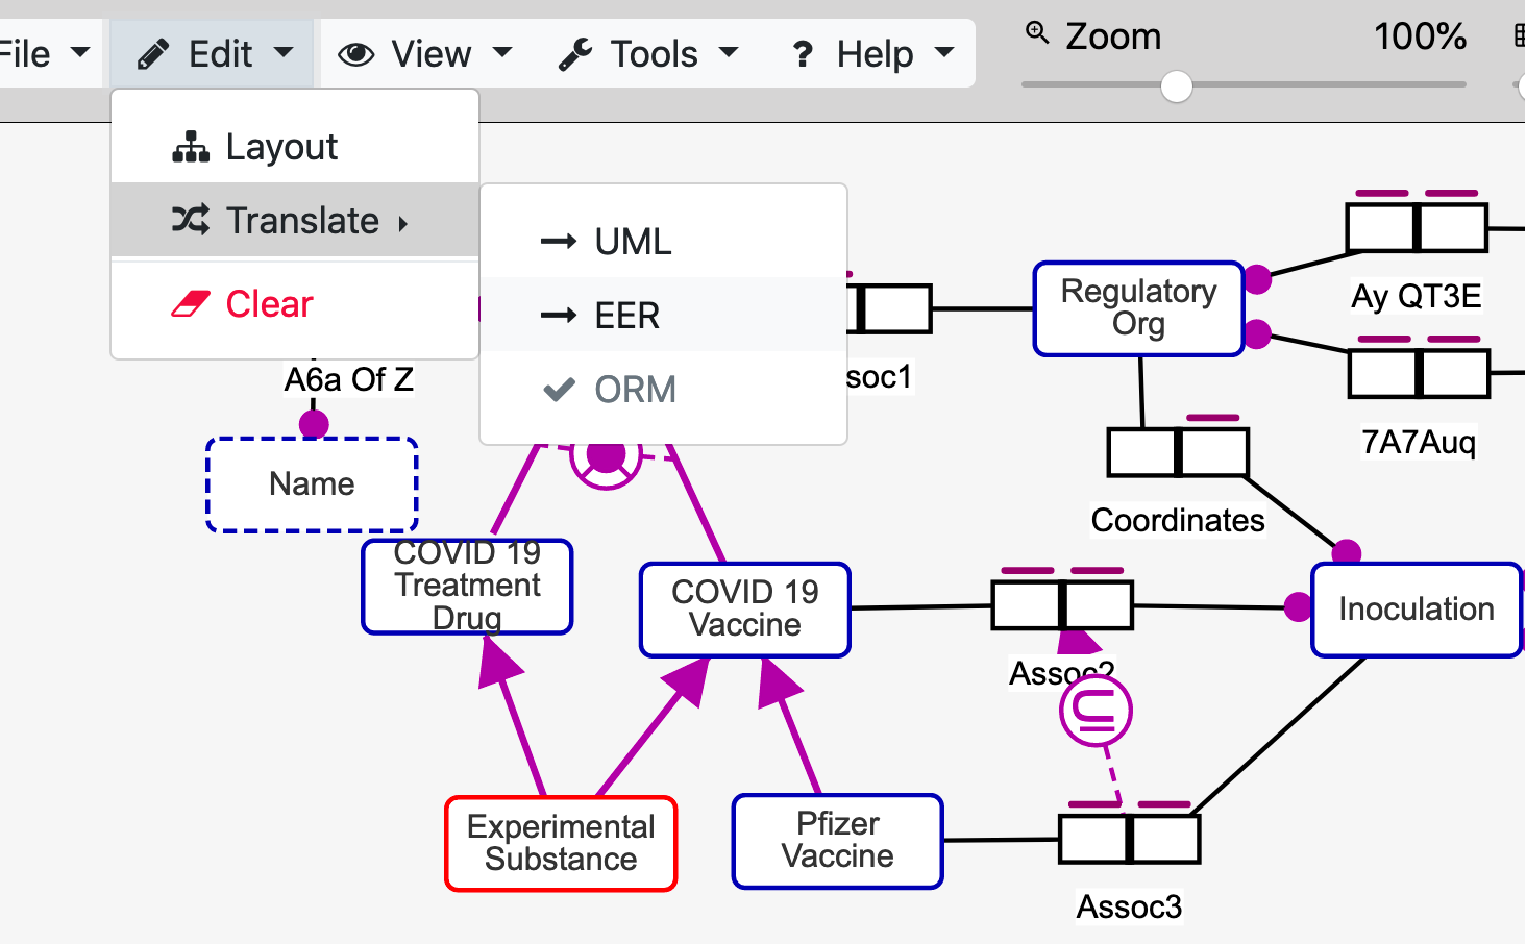
\includegraphics[width=0.95\textwidth]{covidORM2toER2.pdf} 
            
      \vspace{1mm}
      
            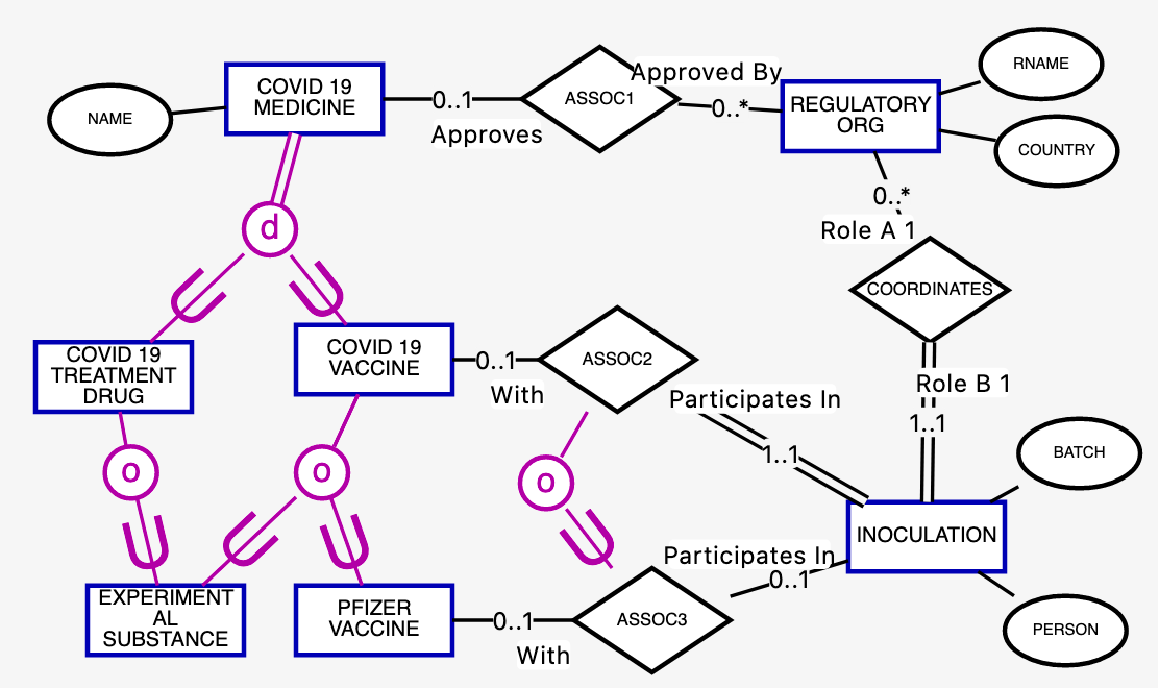
\includegraphics[width=0.95\textwidth]{covidER2.pdf} 
    \caption{With the  {\sf Pfizer vaccine} cardinality deduction accepted and the model updated, the intent is to swap back to EER notation (top) and the outcome of that (bottom).}
    \label{fig:ORM2toER}
\end{figure}

\begin{figure}[h]
  \centering
      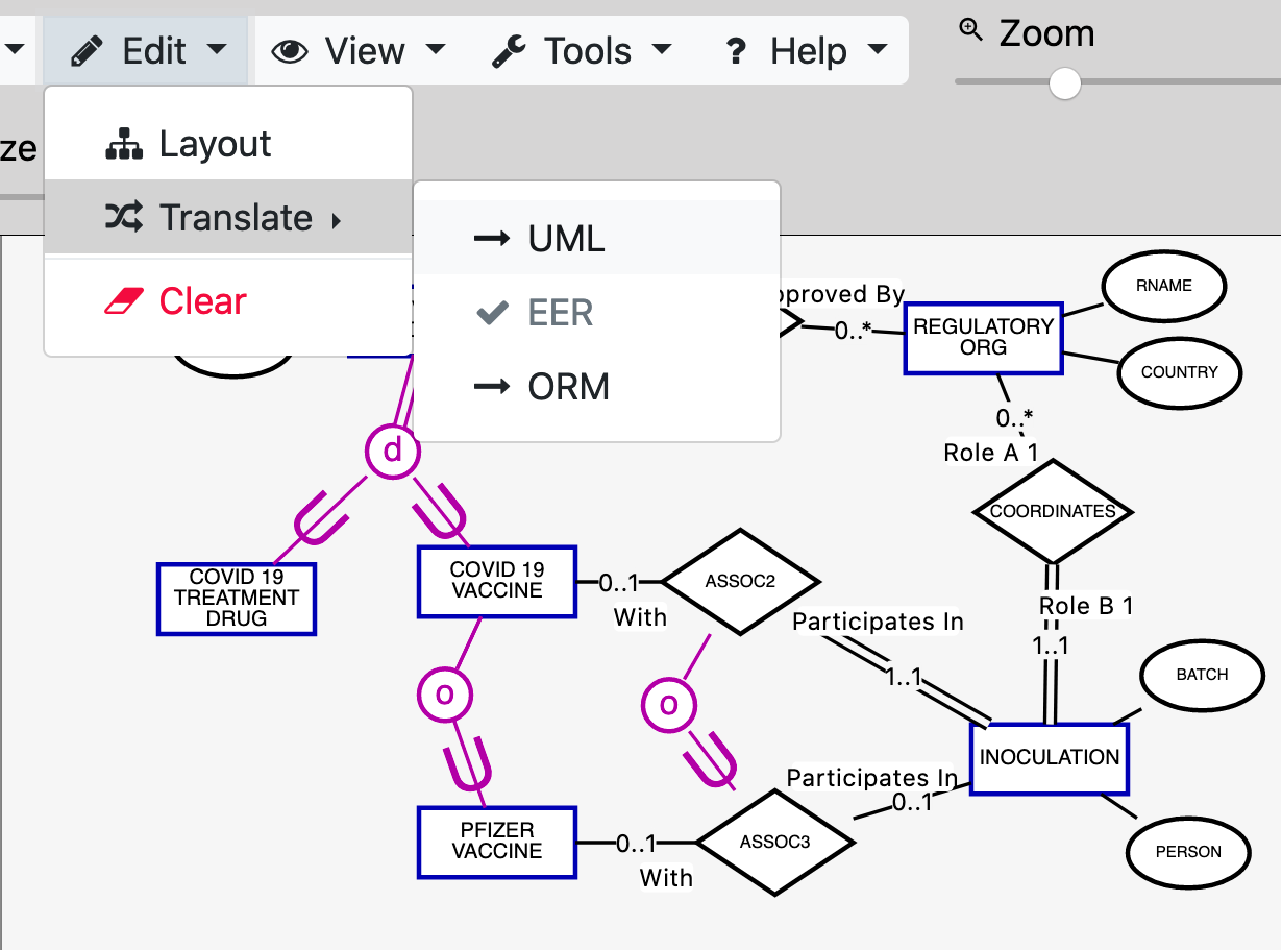
\includegraphics[width=0.95\textwidth]{covidER2toUML.pdf} 
    \caption{With the unsatisfiable class removed, the intent is to swap back to UML notation again.}
    \label{fig:ER2toUML}
\end{figure}

\begin{figure}[h]
  \centering
      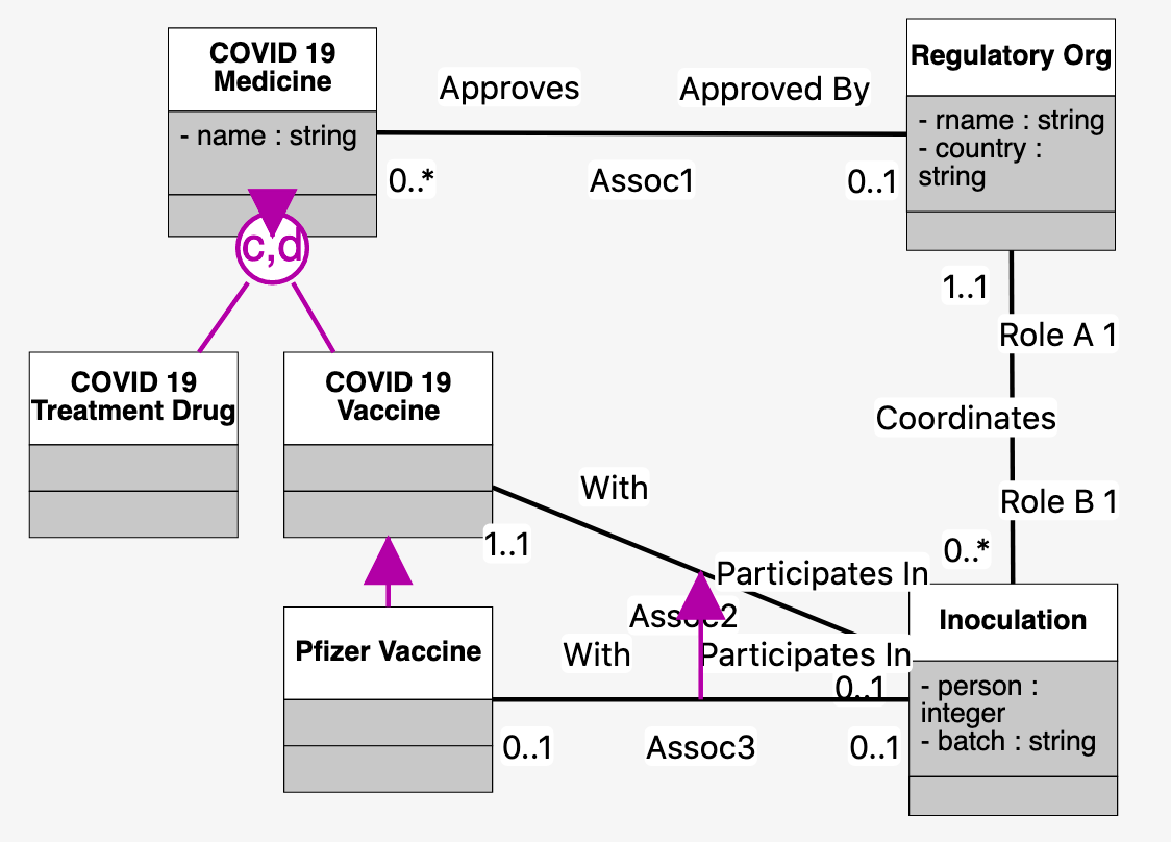
\includegraphics[width=0.95\textwidth]{covidUML3.pdf} 
            
      \vspace{1mm}
      
            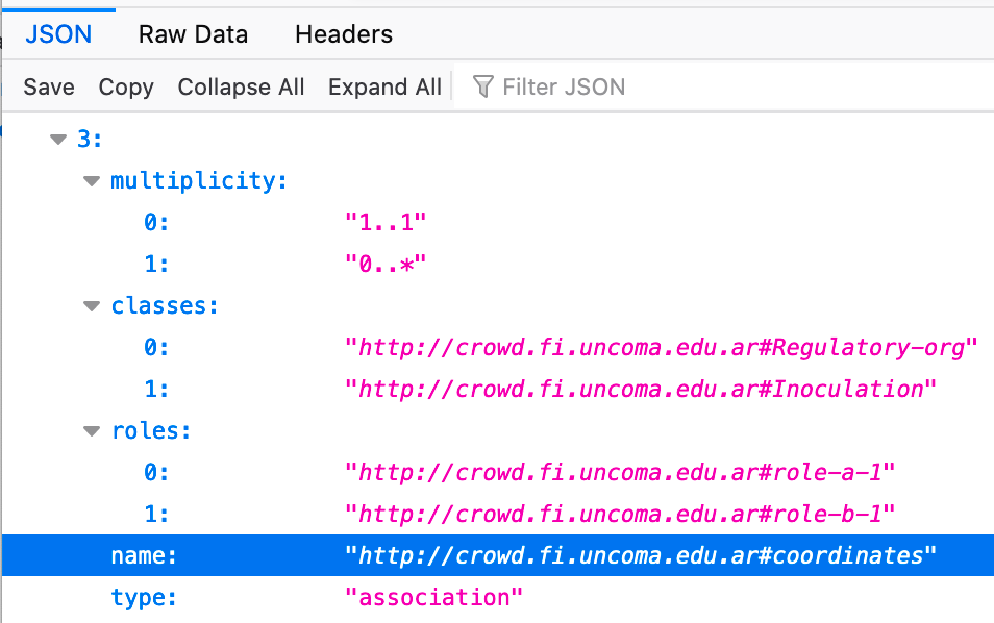
\includegraphics[width=0.95\textwidth]{covidUML3json.pdf} 
    \caption{Back in UML, maintaining that named association (top), which is also reflected in the runtime conceptual model and therefore also its exported serialisation in JSON (bottom).}
    \label{fig:UMLmod}
\end{figure}

\begin{figure}[h]
  \centering
      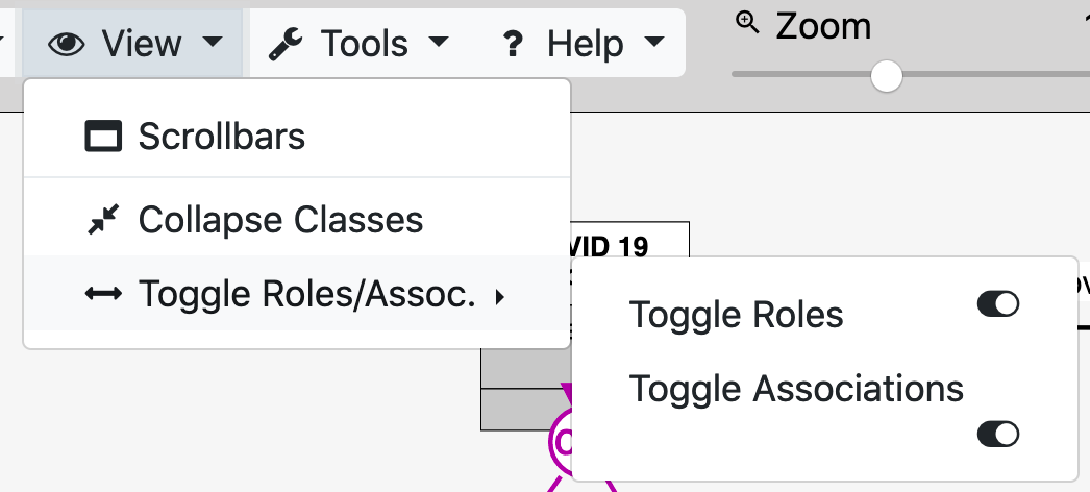
\includegraphics[width=0.95\textwidth]{toggleRR.pdf} 
            
      \vspace{1mm}
      
            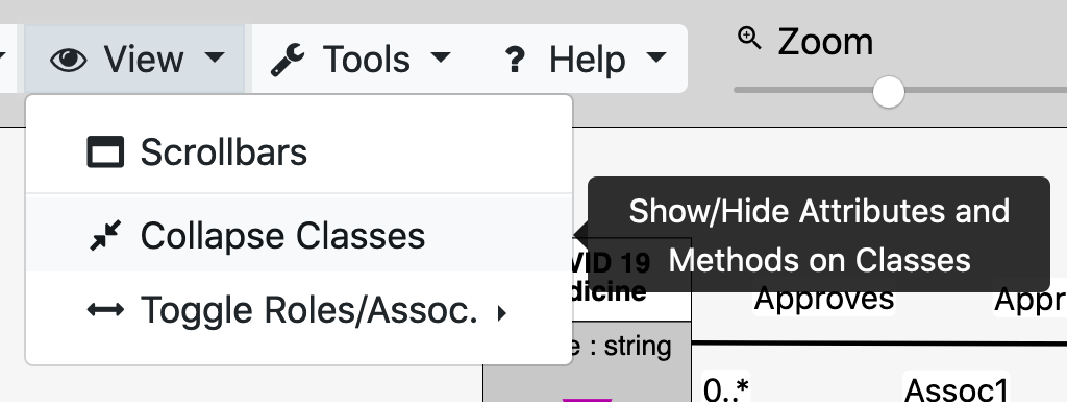
\includegraphics[width=0.95\textwidth]{showhideAtt.pdf} 
            
                  \vspace{1mm}
      
            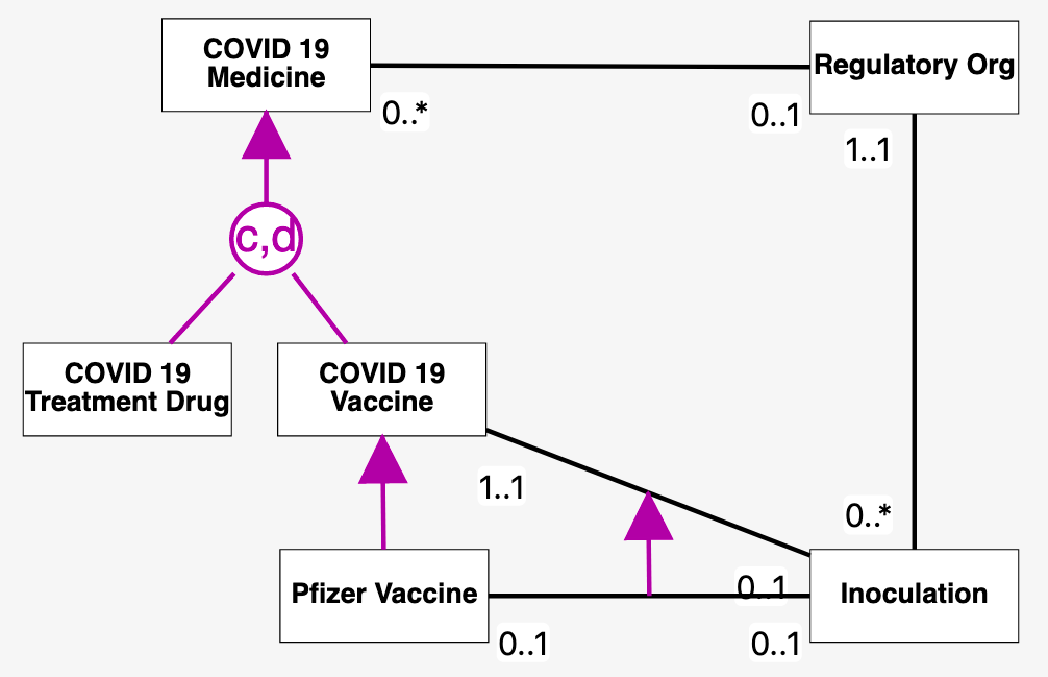
\includegraphics[width=0.95\textwidth]{UML3clean.pdf} 
    \caption{Toggling to abstract away details and generate a simplified view of the same UML diagram as in Fig.~\ref{fig:UMLmod}.}
    \label{fig:UMLabstract}
\end{figure}

\begin{figure}[h]
  \centering
      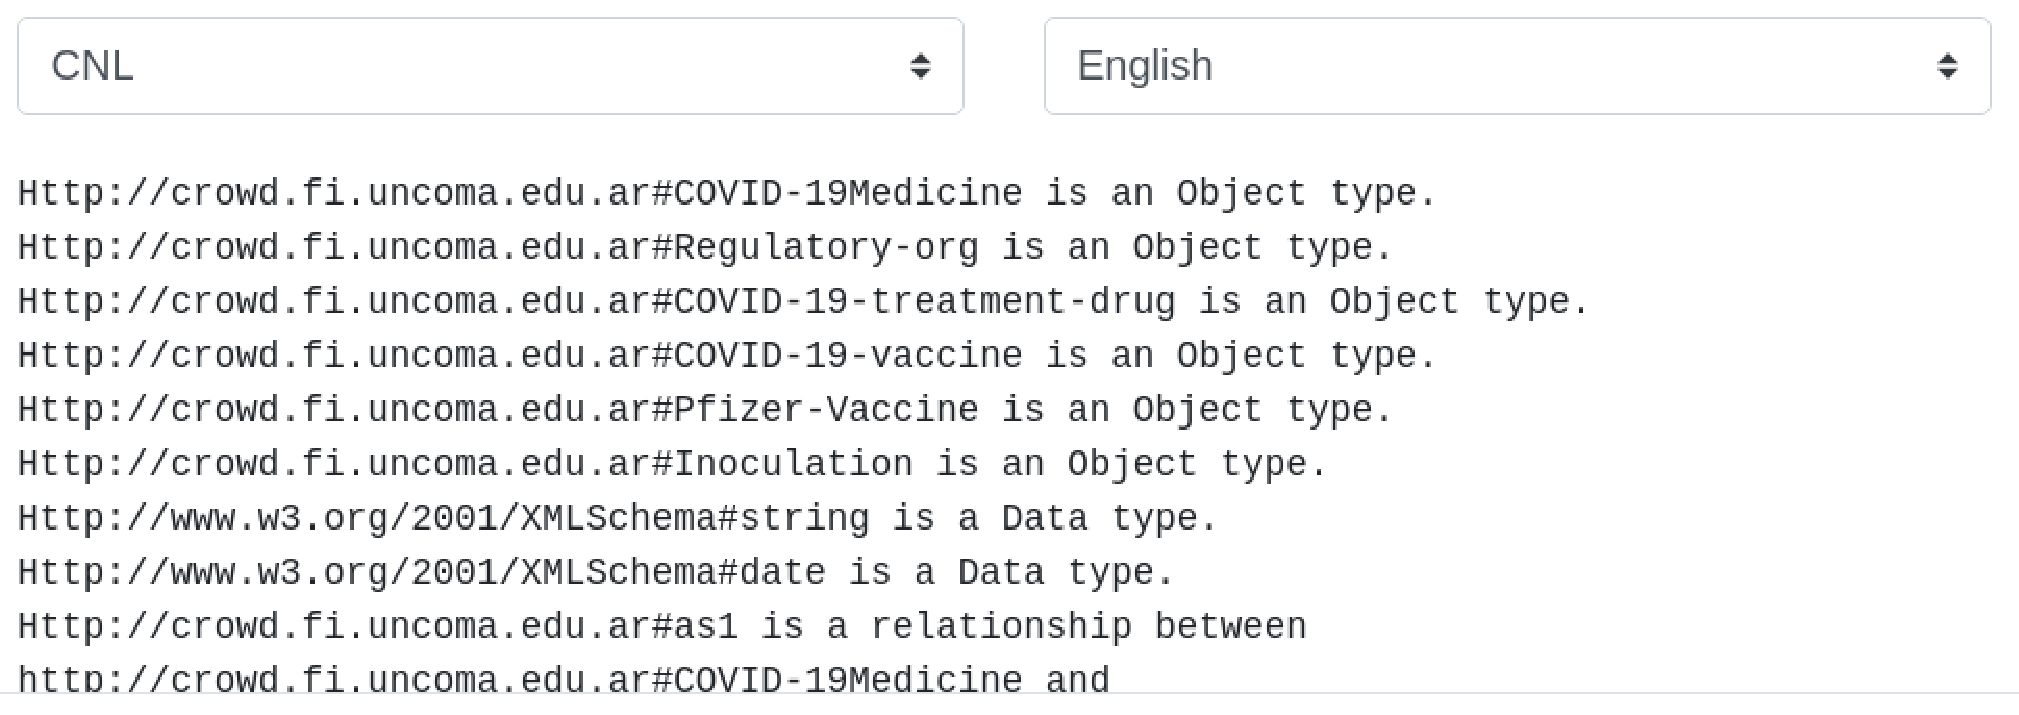
\includegraphics[width=1.0\textwidth]{covid19-cnl.pdf} 
    \caption{Screenshot of a section of the CNL output for the final model.}
    \label{fig:toCNL}
\end{figure}



\begin{figure}[h]
  \centering
      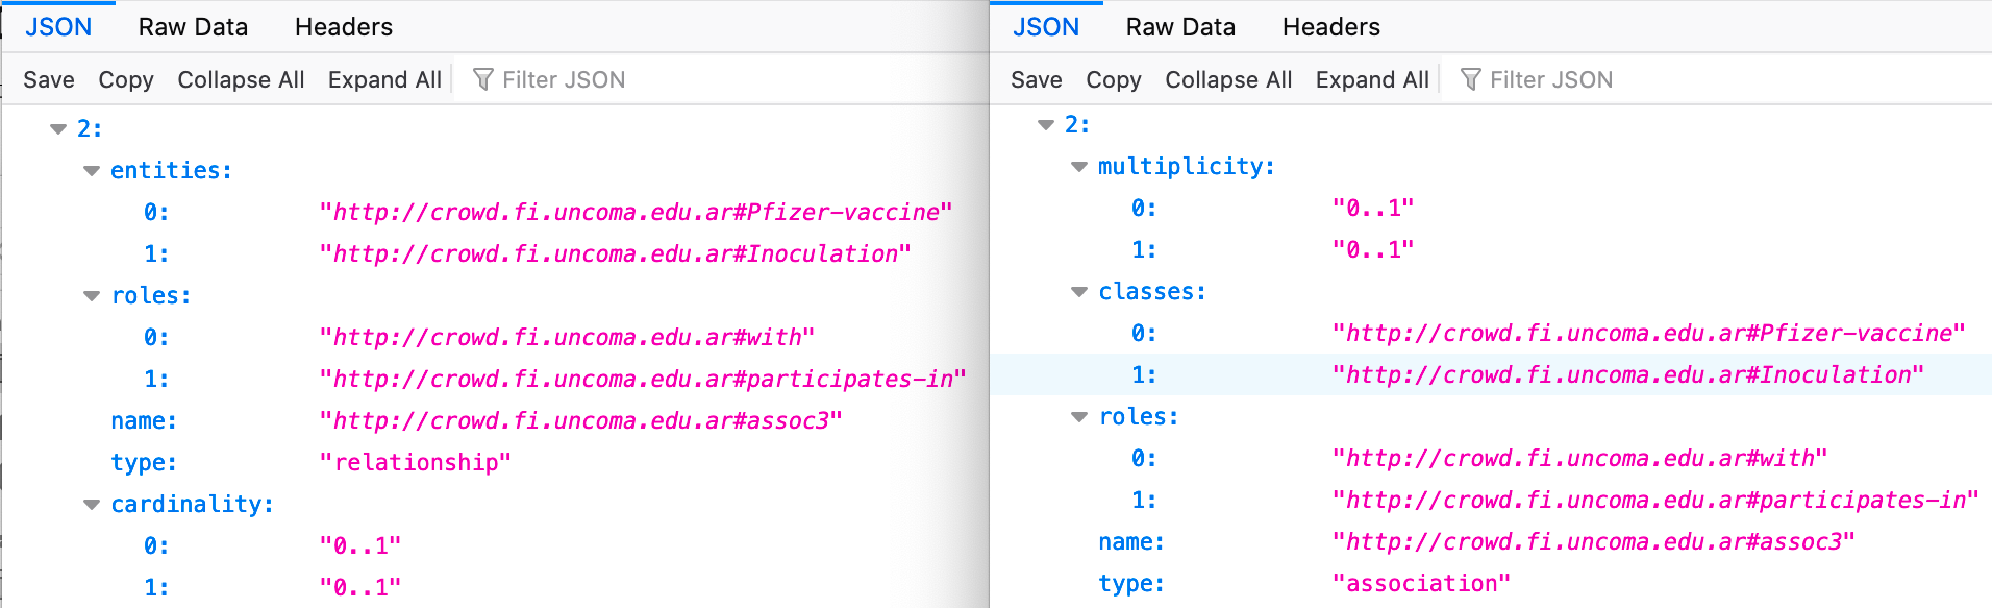
\includegraphics[width=1.0\textwidth]{covidER2andUML2export.pdf} 
    \caption{Screenshots of comparable sections of the respective JSON file that is specific to each CDML. Left: EER; Right: UML}
    \label{fig:jsonER2andUML2}
\end{figure}


\begin{figure}[h]
  \centering
      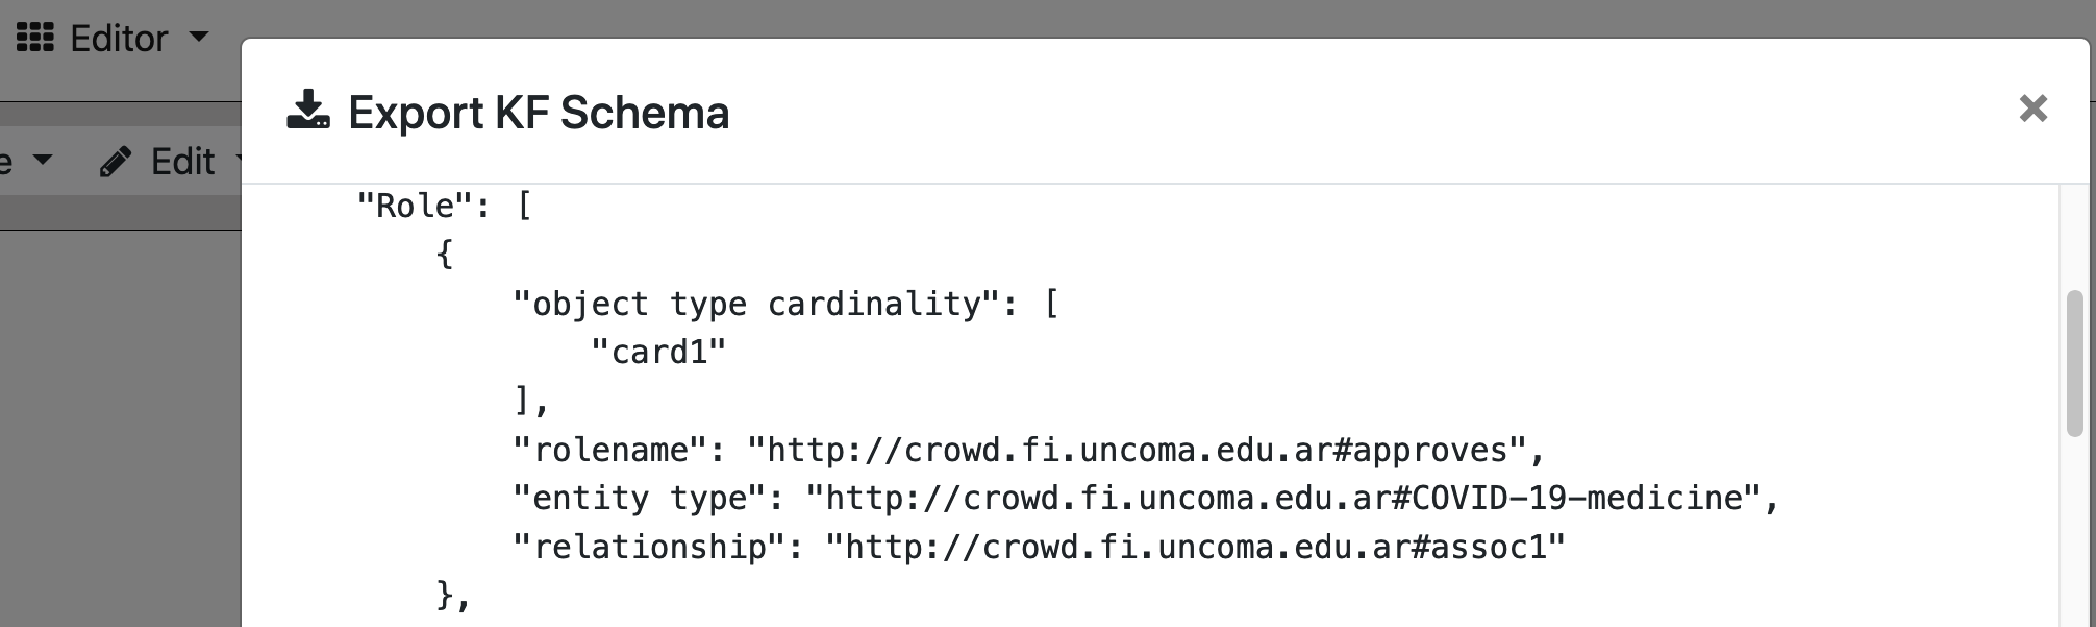
\includegraphics[width=1.0\textwidth]{covidexportKF.pdf} 
    \caption{Screenshot of the export to the KF metamodel persistent storage.}
    \label{fig:toKF}
\end{figure}


\begin{figure}[h]
  \centering
      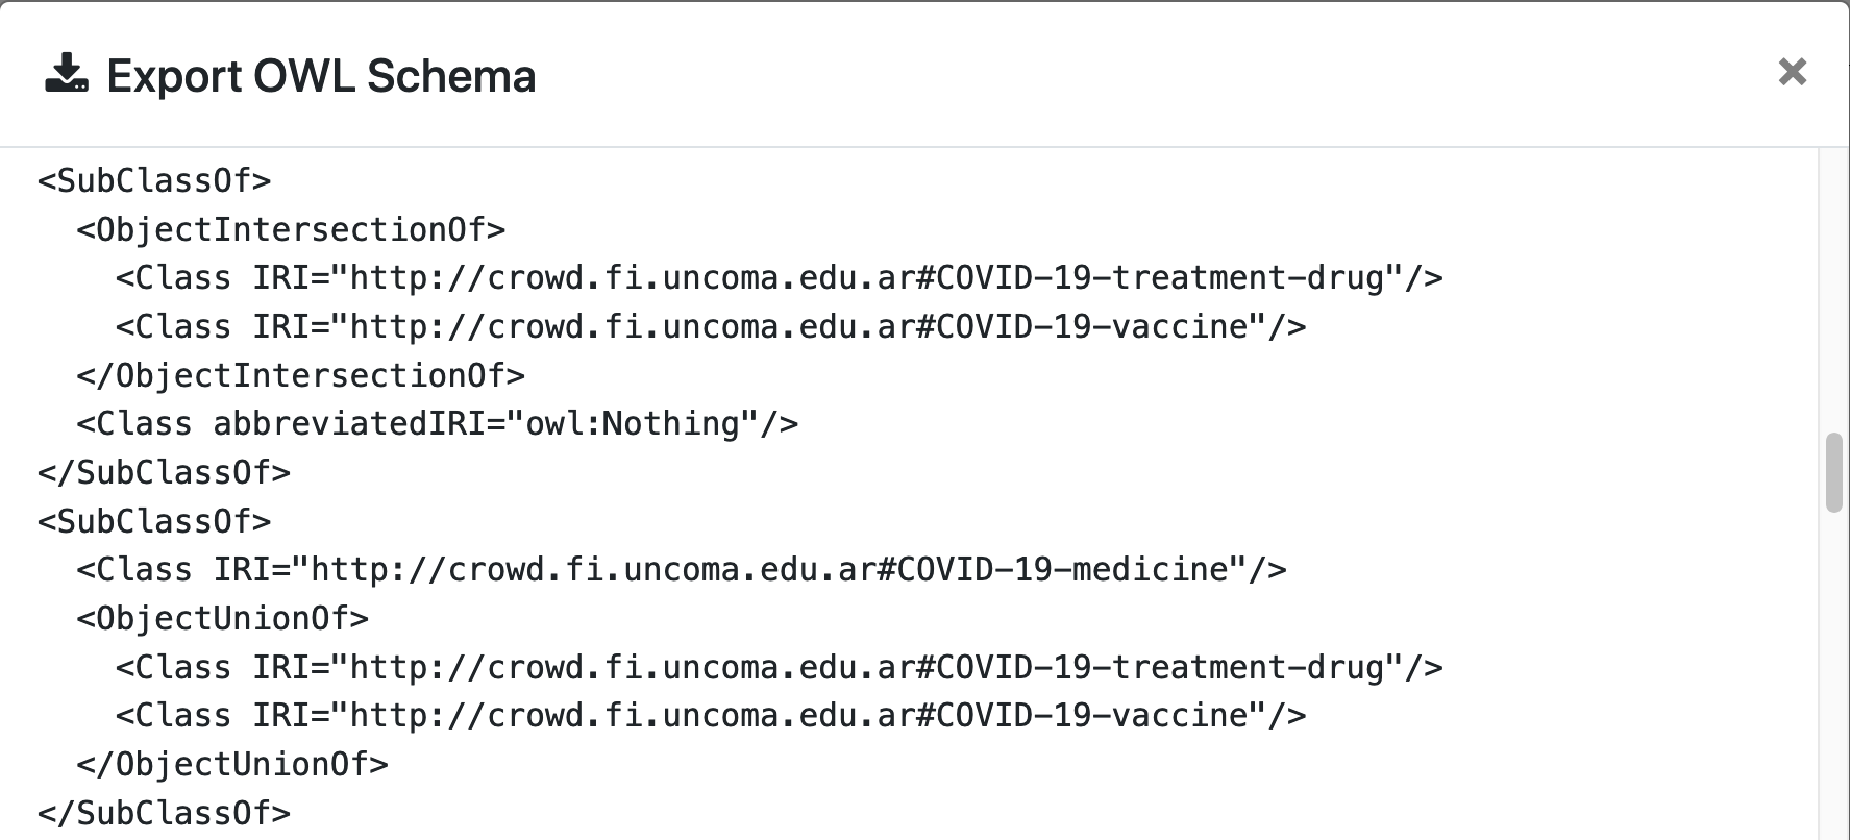
\includegraphics[width=1.0\textwidth]{covidexporttoOWL.pdf} 
    \caption{Screenshot of the KF metamodel encoded into OWL/XML format, at the time of exporting it for use elsewhere.}
    \label{fig:toOWL}
\end{figure}




\end{document}

